%%%%%%%%%%%%%%%%%%%%%%%%%%%%%%%%%%%%%%%%%
% Minimalist Book Title Page 
% LaTeX Template
% Version 1.0 (27/12/12)
%
% This template has been downloaded from:
% http://www.LaTeXTemplates.com
%
% Original author:
% Peter Wilson (herries.press@earthlink.net)
%
% License:
% CC BY-NC-SA 3.0 (http://creativecommons.org/licenses/by-nc-sa/3.0/)
% 
% Instructions for using this template:
% This title page compiles as is. If you wish to include this title page in 
% another document, you will need to copy everything before 
% \begin{document} into the preamble of your document. The title page is
% then included using \titleTH within your document.
%
%%%%%%%%%%%%%%%%%%%%%%%%%%%%%%%%%%%%%%%%%

%----------------------------------------------------------------------------------------
%	PACKAGES AND OTHER DOCUMENT CONFIGURATIONS
%----------------------------------------------------------------------------------------

\documentclass[a4paper,10.9pt]{article}
\usepackage{pdfpages}
\usepackage{fancyhdr}
\usepackage{nth}
\usepackage[utf8]{inputenc}


\setlength{\parindent}{4em}
\setlength{\parskip}{1em}
\renewcommand{\baselinestretch}{1.5}

%booleanclaration
\newboolean{twoside}
\setboolean{twoside}{false}
\usepackage[landscape,twocolumn]{geometry}
 \geometry{
 a4paper,
 total={170mm,257mm},
 left=20mm,
 top=20mm,
 }

\newenvironment{dedication}
{
   \cleardoublepage
   \thispagestyle{empty}
   \vspace*{\stretch{1}}
   \hfill\begin{minipage}[t]{0.66\textwidth}
   \raggedright
}%
{
   \end{minipage}
   \vspace*{\stretch{3}}
   \clearpage
}



%----------------------------------------------------------------------------------------
%	BLANK DOCUMENT
%----------------------------------------------------------------------------------------

\begin{document} 
 \thispagestyle{empty}
%________________New Section // Score
\begin{figure}
\section{A Way After The Fox's Backbone}
\end{figure}
\begin{figure}
\subsection{Two Types of Space}
Real physical proportions are translated into abstract representations and related to duration. 
\begin{center}
 \includegraphics[width=8cm]{./Precompile/FOX-FormSketch.png}
\caption{Sketch of Time Structure}
\end{center}
\end{figure}
\hspace{10cm}
\begin{figure}
\subsection{Realist Composition}
Multiple perspectives are drawn independently and combined to create a dialogue within the picture plane. 
\begin{center}
 \includegraphics[width=8cm]{./Precompile/Van_Eyck_-_Arnolfini_Portrait.jpg}
\caption{Arnolfini Portrait -- Jan van Eyck}
\end{center}
\end{figure}
\pagebreak
\thispagestyle{empty} 
\begin{figure}
\subsection{Instrumental Technique}
The outline of the skeleton represents the harmonic and tonal backbone of the piece,
musical material that acts as an opaque base, reflecting harmony through the layers of instrumental sound. 

\begin{center}
 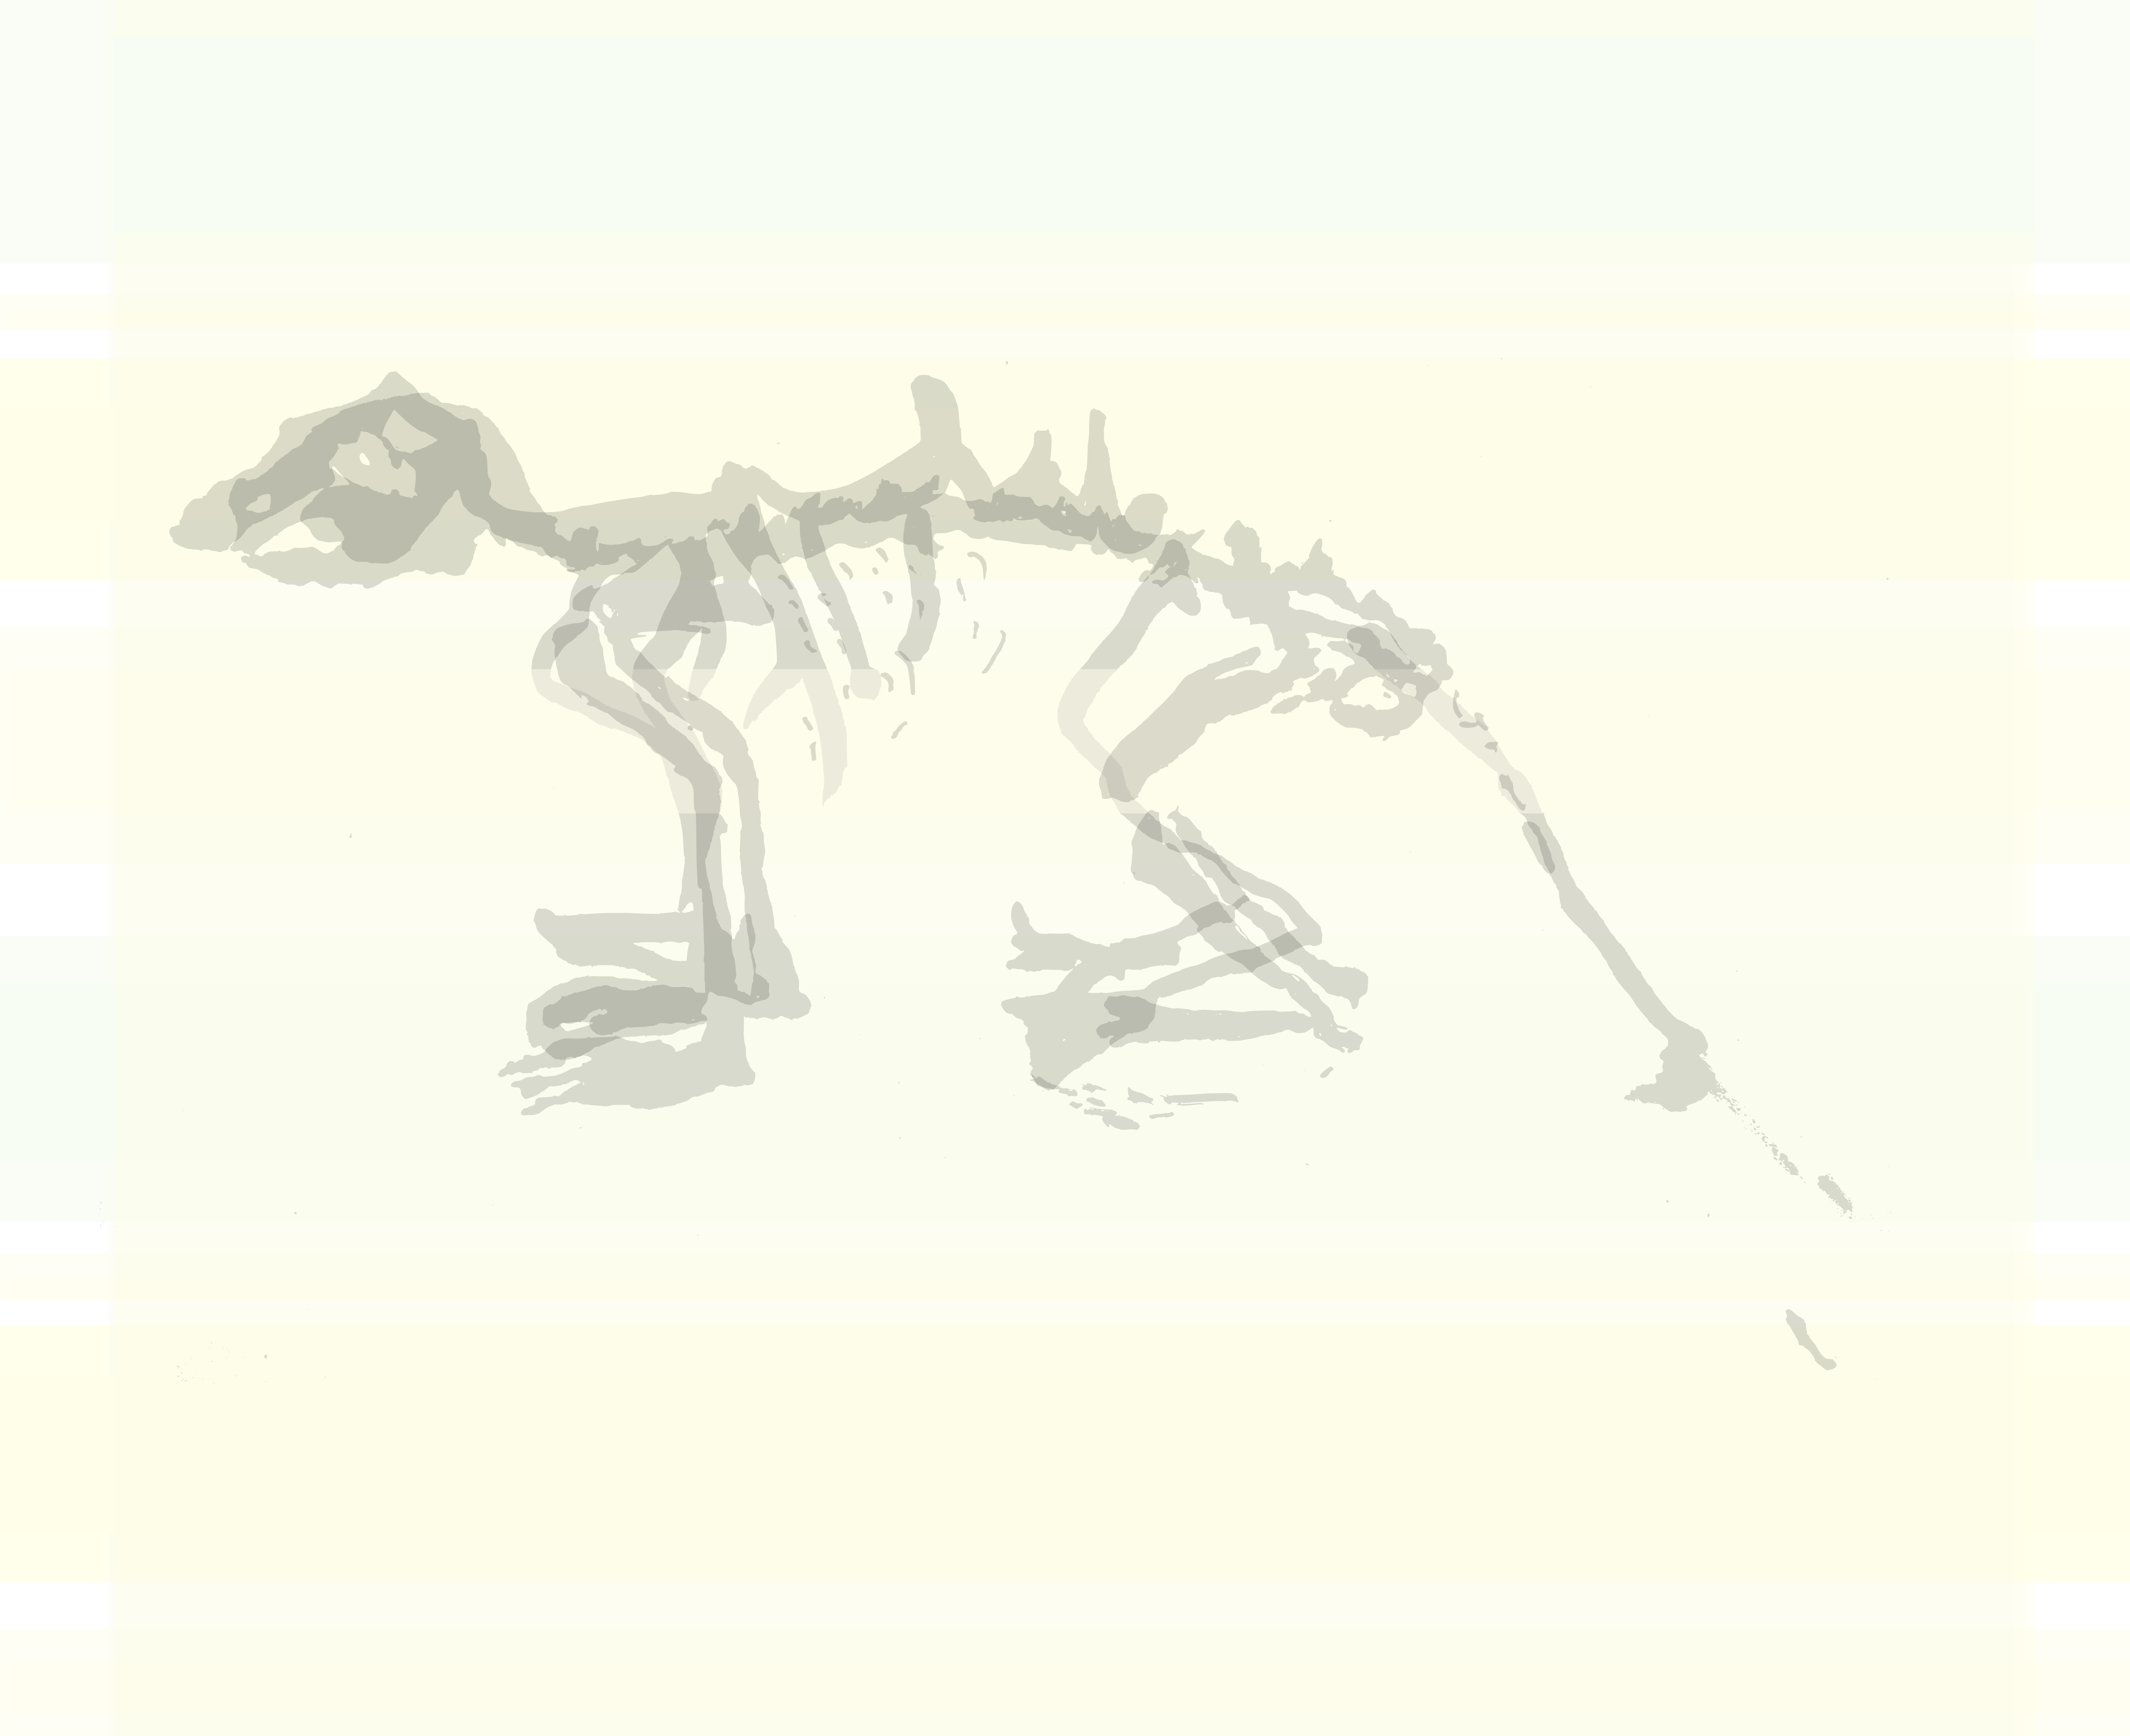
\includegraphics[width=8cm]{./Precompile/FOX6a.png}
\caption{Sketch of Orchestration}
\end{center}
\end{figure}

\end{document}